% \section{Đặc tả các lược đồ}
% \subsection{Các use-case và các kịch bản}
\subsection{Thiết kế class diagram}

\begin{figure}[H]
    \centering
    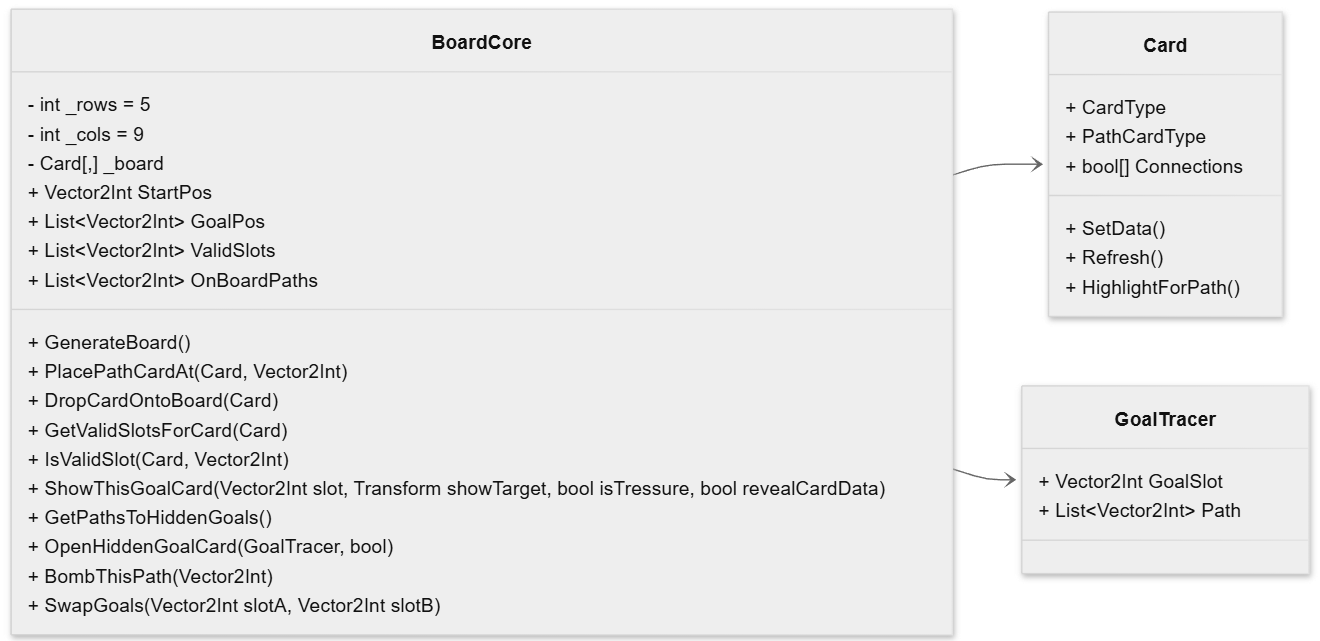
\includegraphics[width=0.9\linewidth]{9.Đặc tả các lược đồ/diagram/board_core.png} 
    \caption{Board Core}
    \label{fig:placeholder}
\end{figure}
\textbf{BoardCore} là thành phần cốt lõi quản lý logic bàn cờ trong trò chơi. Lớp chịu trách nhiệm khởi tạo bàn cờ (GenerateBoard), đặt và kiểm tra vị trí các lá bài đường đi, quản lý các mục tiêu ẩn, cùng các chức năng đặc biệt như phá đường và hoán đổi thẻ dích,... Lớp tương tác chặt chẽ với lớp \textbf{Card} và \textbf{GoalTracer} để xử lý kết nối đường đi và tương tác với thẻ dích.

\begin{figure}[H]
    \centering
    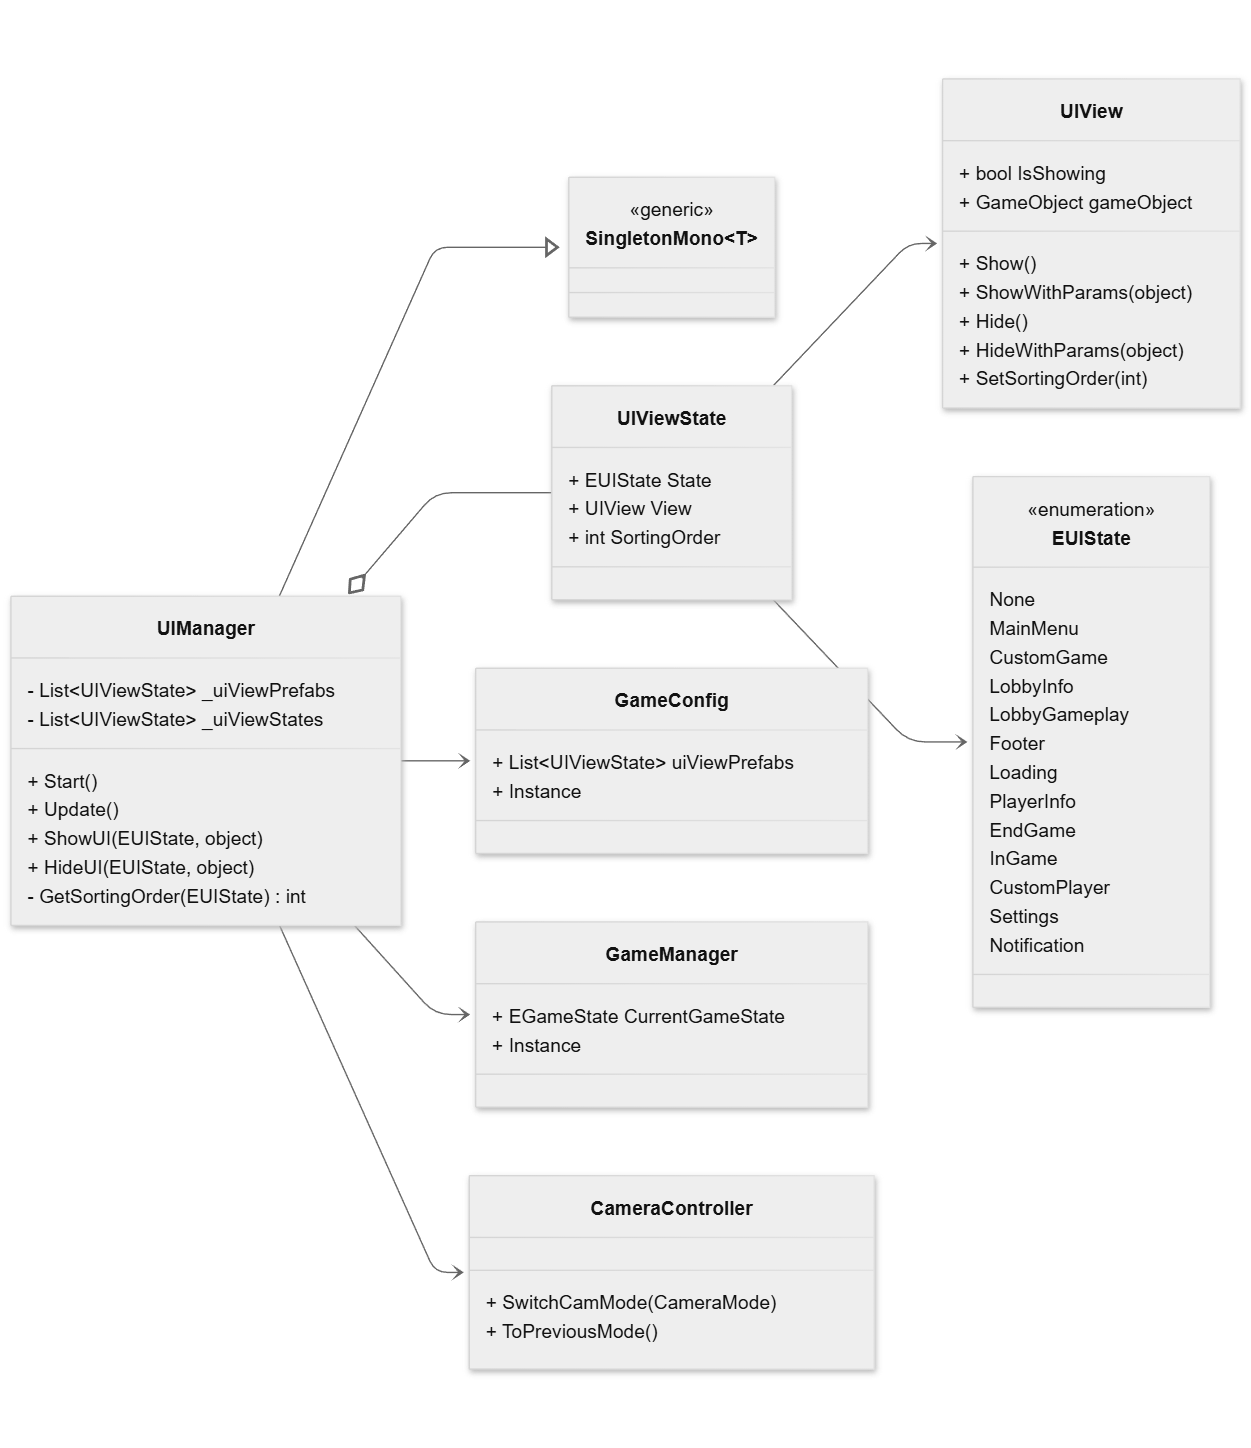
\includegraphics[width=0.9\linewidth]{9.Đặc tả các lược đồ/diagram/UIManager.png}
    \caption{UI Manger}
    \label{fig:placeholder}
\end{figure}
\textbf{UIManager} kế thừa từ \textit{SingletonMono} chịu trách nhiệm quản lý và hiển thị các giao diện người dùng theo trạng thái (EUIState). Lớp sử dụng cơ chế UIViewState và UIView để kiểm soát việc show/hide các giao diện, sắp xếp thứ tự (sorting order).

\begin{figure}[H]
    \centering
    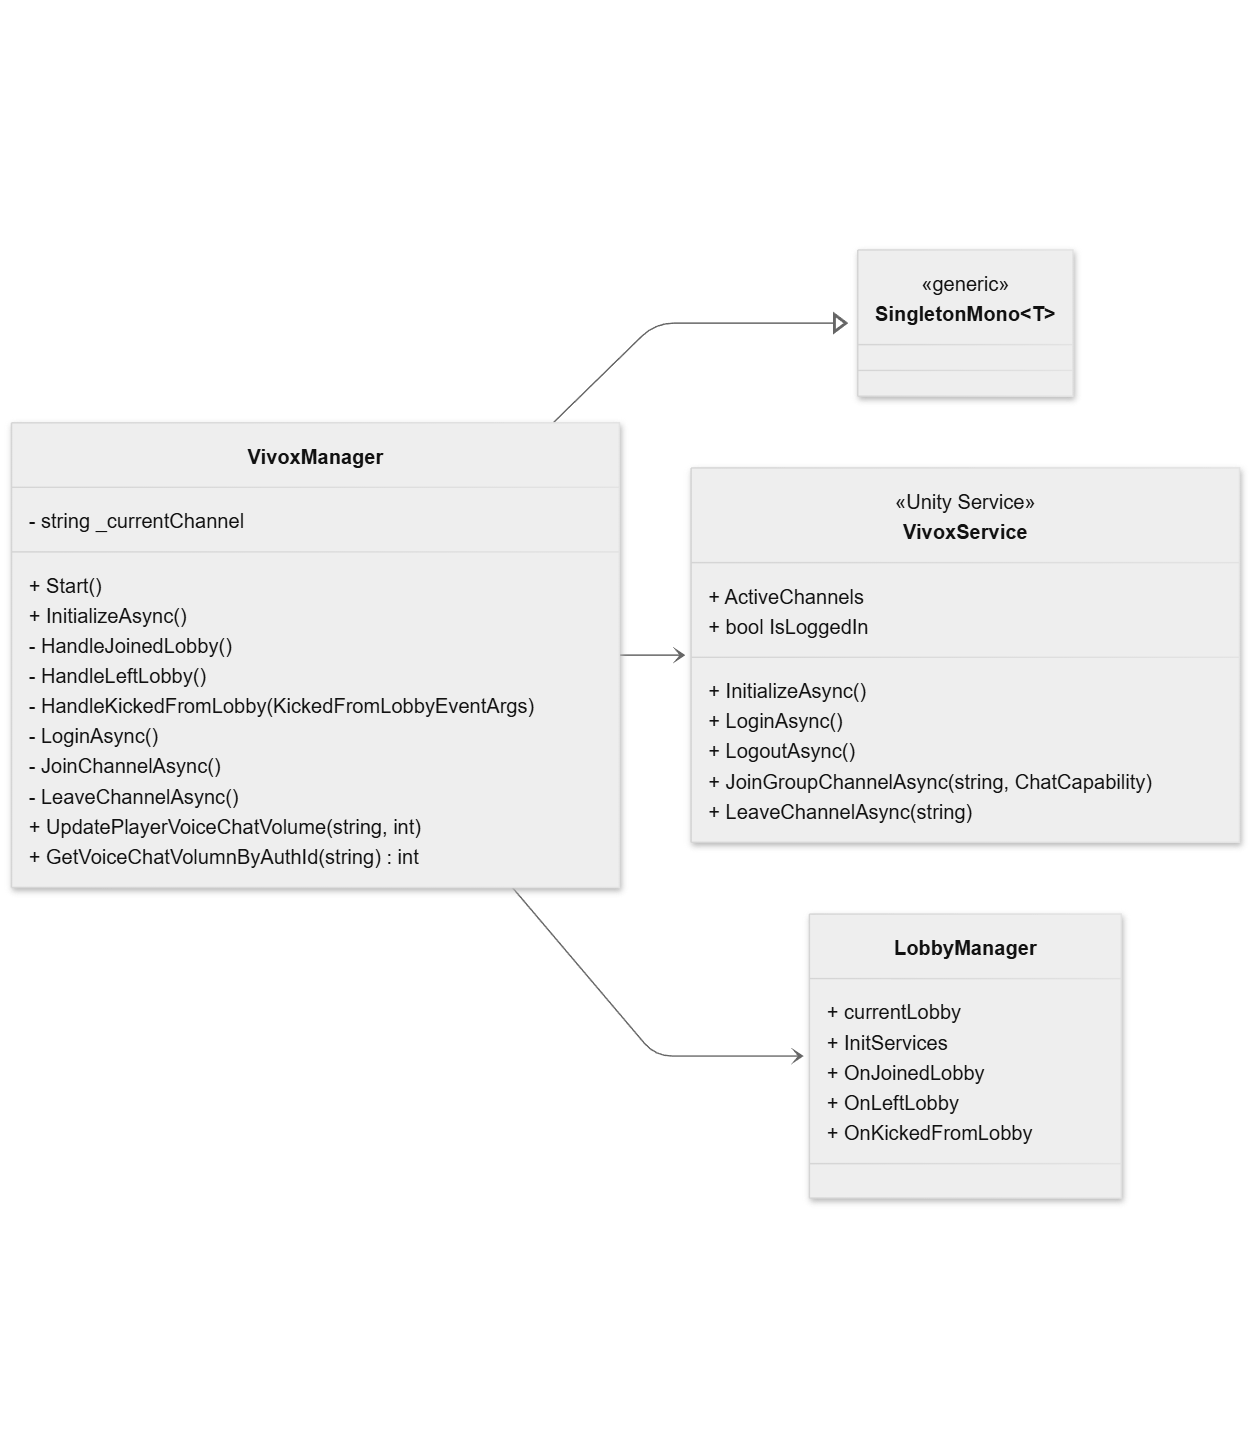
\includegraphics[width=0.9\linewidth]{9.Đặc tả các lược đồ//diagram/vivox_voice_manager.png}
    \caption{Vivox Voice Manager}
    \label{fig:placeholder}
\end{figure}
\textbf{VivoxManager} kế thừa từ \textit{SingletonMono} quản lý hệ thống voice-text chat trong trò chơi. Lớp xử lý việc đăng nhập Vivox, tham gia/rời kênh thoại theo lobby, và điều chỉnh âm lượng giọng nói của từng người chơi.

\noindent
\begin{figure}[H]
    \centering
    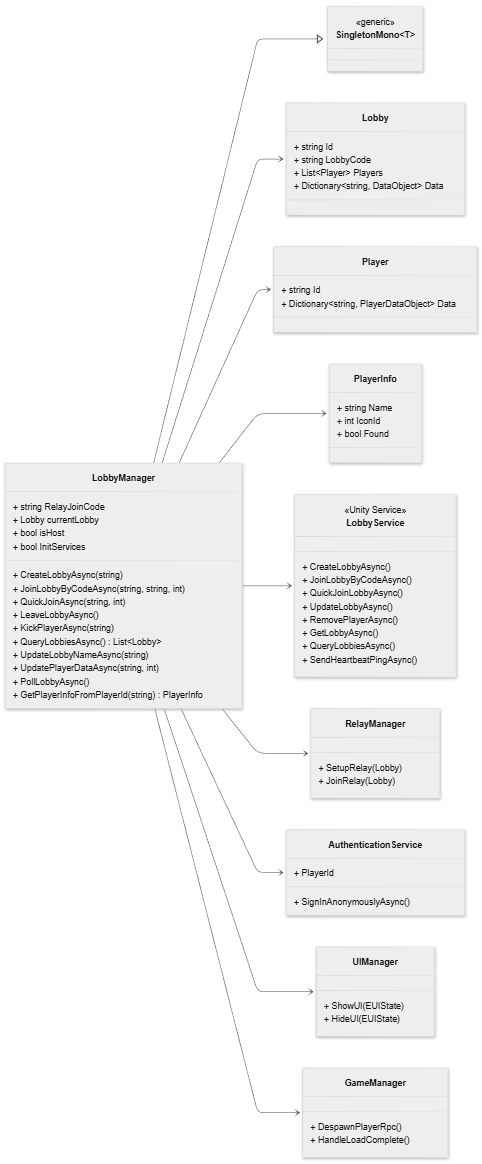
\includegraphics[width=0.5\linewidth]{9.Đặc tả các lược đồ//diagram/lobby_manager.png}
    \caption{Lobby Manager}
    \label{fig:placeholder}
\end{figure}
\textbf{LobbyManager} kế thừa từ \textit{SingletonMono} chịu trách nhiệm quản lý toàn bộ các chức năng liên quan đến lobby. Lớp cung cấp các phương thức bất đồng bộ để tạo lobby, tham gia lobby (quick join hoặc bằng code), cập nhật thông tin lobby, kick người chơi và tích hợp Relay để kết nối mạng. Lớp tương tác chặt chẽ với \textit{LobbyService}, \textbf{RelayManager} và \textit{AuthenticationService} của Unity.

\begin{figure}[H] 
    \centering
    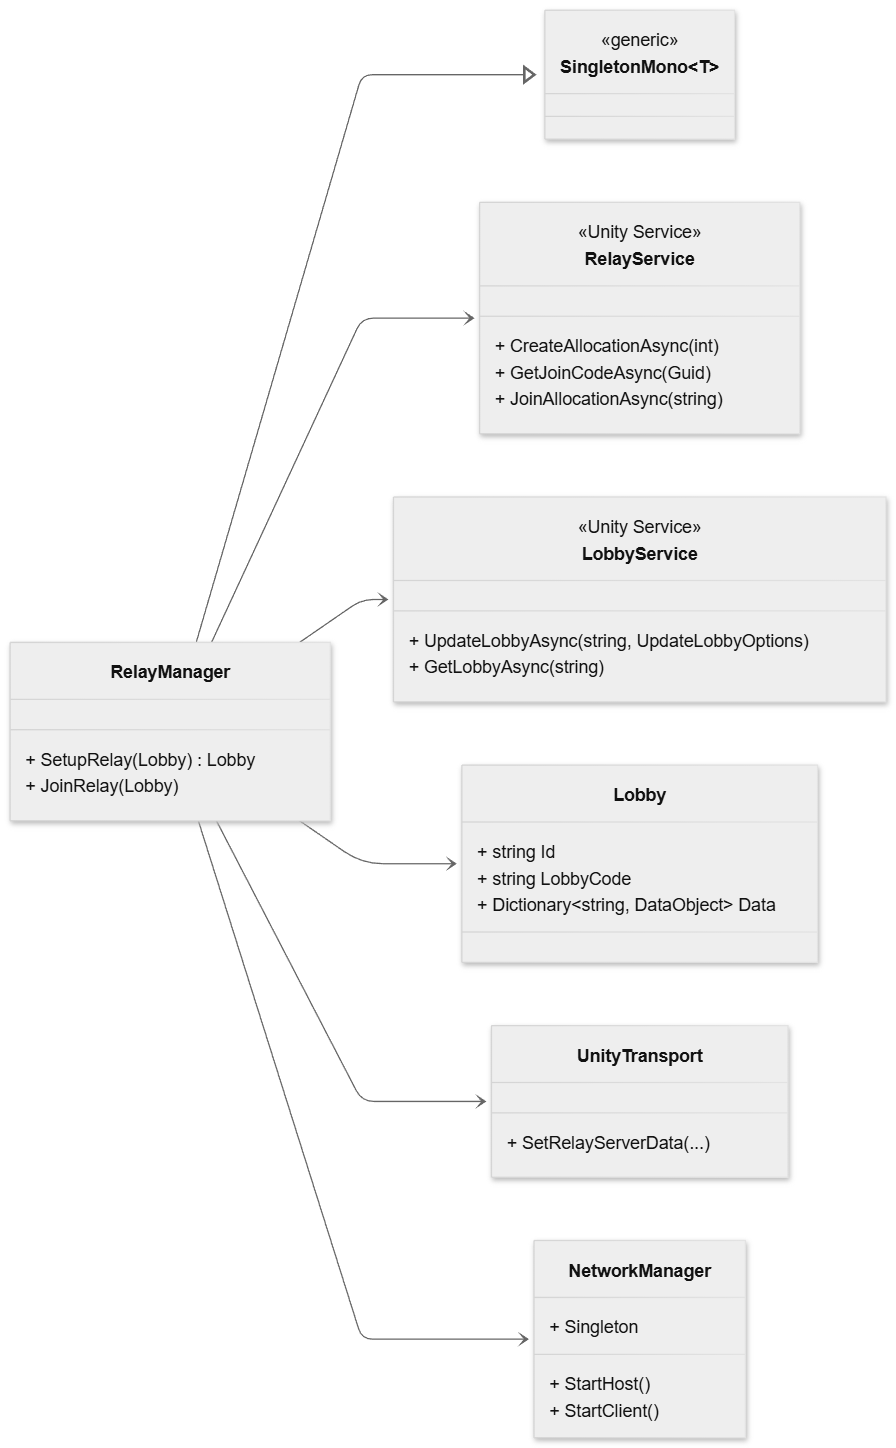
\includegraphics[width=0.6\linewidth]{9.Đặc tả các lược đồ//diagram/relay_manager.png}
    \caption{Relay Manager}
    \label{fig:placeholder}
\end{figure}
\textbf{RelayManager} kế thừa từ \textit{SingletonMono} chịu trách nhiệm thiết lập và quản lý kết nối Relay của Unity để hỗ trợ giao tiếp mạng P2P. Lớp cung cấp các chức năng SetupRelay và JoinRelay, tương tác với \textit{RelayService} và \textit{LobbyService} nhằm tạo allocation và thiết lập server relay cho các phiên chơi.

\begin{figure}[H]
    \centering
    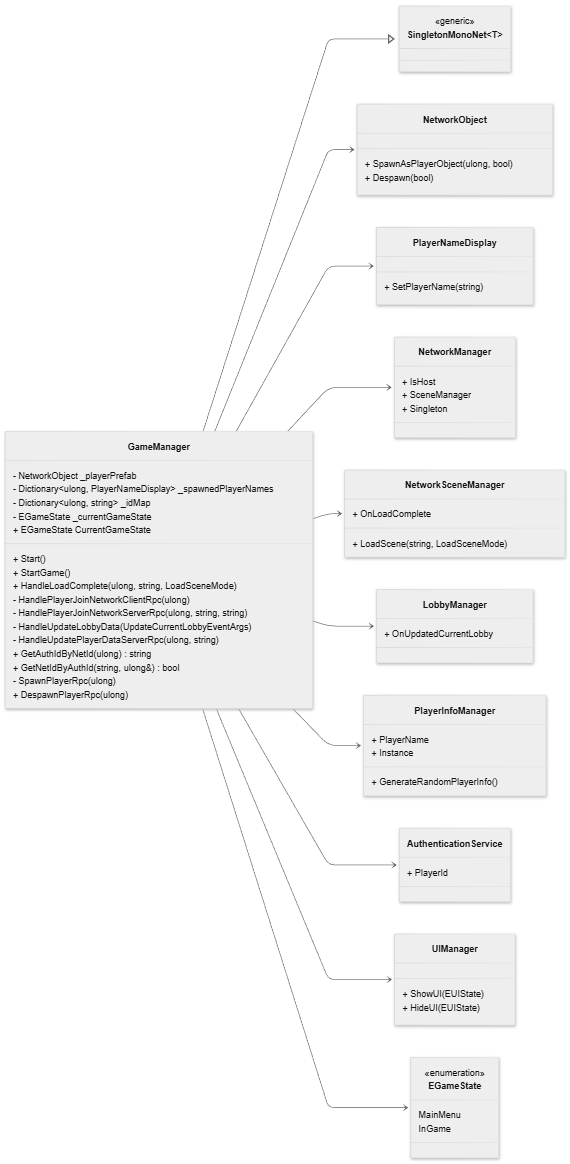
\includegraphics[width=0.5\linewidth]{9.Đặc tả các lược đồ/diagram/game_manager.png}
    \caption{Game Manger}
    \label{fig:placeholder}
\end{figure}
\textbf{GameManager} kế thừa từ \textit{SingletonMonoNet} đóng vai trò trung tâm quản lý trạng thái và vòng đời của trò chơi. Lớp xử lý việc spawn/despawn người chơi, chuyển cảnh, đồng bộ trạng thái lobby và quản lý game state (EGameState). Đây là lớp chính kết nối giữa hệ thống mạng (\textit{NetworkManager}), lobby và giao diện người chơi.
\begin{figure}[H]
    \centering
    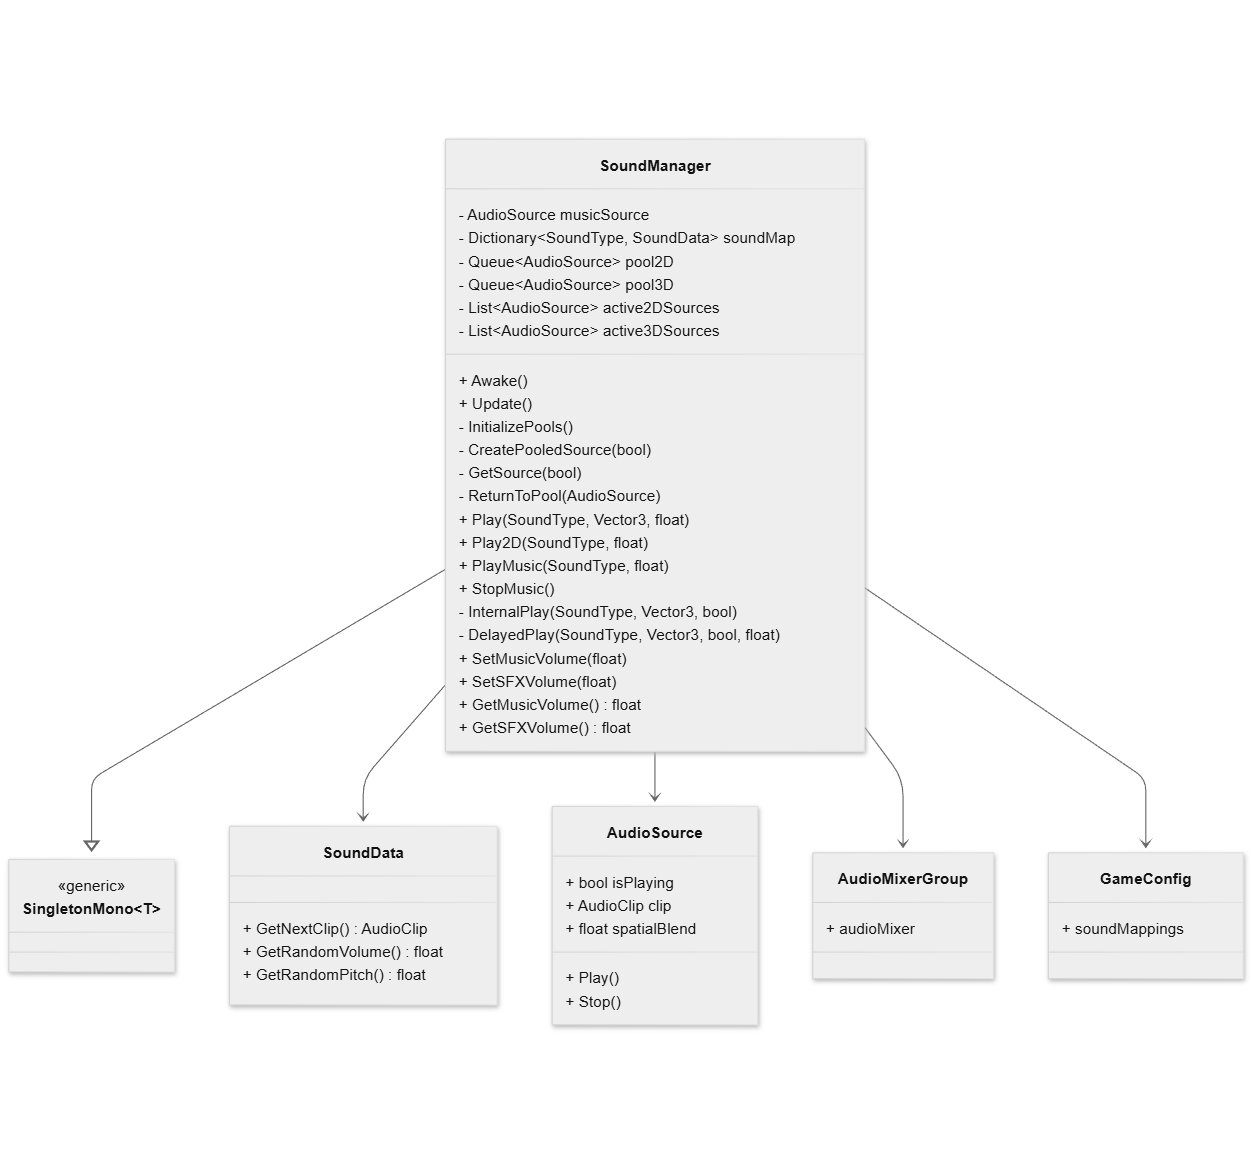
\includegraphics[width=0.9\linewidth]{9.Đặc tả các lược đồ/diagram/sound_manager.png}
    \caption{Sound Manger}
    \label{fig:placeholder}
\end{figure}
\textbf{SoundManager} kế thừa từ \textit{SingletonMono} quản lý hệ thống âm thanh toàn cục của trò chơi. Lớp hỗ trợ phát nhạc nền, hiệu ứng âm thanh 2D/3D với hệ thống object pooling, điều chỉnh âm lượng và quản lý các AudioSource một cách hiệu quả.